\documentclass[journal]{IEEEtran} % or [conference] if you target a conference

% ============================================================================
% CORE PACKAGES (IEEE-style)
% ============================================================================


% ========== REQUIRED PACKAGES (add to preamble) ==========
\usepackage{pgfplots}
\pgfplotsset{compat=1.17}
\usepackage{tikz}
\usetikzlibrary{shapes, arrows}

\usetikzlibrary{shapes, arrows, positioning, calc}
\usepackage{xcolor}
\usepackage{booktabs}
% Recommended by IEEEtran docs for citations
\usepackage{cite} % compressed, sorted numeric refs [web:2][web:8]
\usepackage{tabularx}
% \usepackage{natbib}
\usepackage[square,numbers,sort&compress]{natbib}
% Graphics and Figures
\usepackage{graphicx}
\usepackage{tikz}
\usetikzlibrary{shapes.geometric, arrows.meta, positioning, fit, backgrounds, calc, decorations.pathreplacing, bending}
\tikzset{>={Stealth}}

% Tables
\usepackage{booktabs}    % \toprule, \midrule, \bottomrule
\usepackage{multirow}
\usepackage{multicol}

% Mathematics
\usepackage{amsmath}
\usepackage{amssymb}
\usepackage{bm}
\usepackage{balance}
% Algorithms and Pseudocode
\usepackage{algorithm}
\usepackage{algorithmicx}
\usepackage{algpseudocode}
\usepackage{algcompatible}
% \usepackage{algorithmic} % IEEEtran-friendly (instead of algpseudocode)

% Colors and Highlighting
\usepackage{xcolor}
\usepackage{soul}        % \hl{}
\usepackage{tcolorbox}   % colored boxes for findings


% Lists and Enumeration
\usepackage{enumitem}
\setlist{nosep}

% Hyperlinks and Clever References
\usepackage[hidelinks]{hyperref}
\usepackage[nameinlink]{cleveref}

% Miscellaneous
\usepackage{url}
\usepackage{xspace}
\usepackage{comment}

% (Optional) Units and Numbers – if you actually use siunitx
\usepackage{siunitx}
\sisetup{
  output-exponent-marker=\ensuremath{\mathrm{e}},
  group-separator={,},
  detect-weight=true,
  detect-inline-weight=math
}

% ============================================================================
% COLOR DEFINITIONS
% ============================================================================

\definecolor{networkblue}{RGB}{52,152,219}
\definecolor{envgreen}{RGB}{46,204,113}
\definecolor{algorange}{RGB}{230,126,34}
\definecolor{allocpurple}{RGB}{155,89,182}

\definecolor{findingBlue}{RGB}{230,240,255}
\definecolor{findingRed}{RGB}{255,230,230}
\definecolor{findingOrange}{RGB}{255,245,230}
\definecolor{findingGreen}{RGB}{230,255,240}

% ============================================================================
% CUSTOM COMMANDS
% ============================================================================
% \algnewcommand\algorithmicrequire{\textbf{Input:}}
\algnewcommand\Require{\item[\algorithmicrequire]}

\newcommand{\ie}{\emph{i.e.,}\xspace}
\newcommand{\eg}{\emph{e.g.,}\xspace}
\newcommand{\etc}{etc.\xspace}
\newcommand{\etal}{\emph{et~al.}\xspace}

\newcommand{\descStep}[2]{\noindent\textbf{#1:} #2}
\newcommand{\smallTitle}[1]{\vspace{1mm}\noindent\textit{#1:}}
\newcommand{\fillin}[1]{\textcolor{gray}{\emph{[#1]}}}
\newcommand{\metric}[1]{\textsc{#1}}

\newcommand{\pp}{\,\%}
\newcommand{\SEM}{\text{SEM}}
\newcommand{\eff}{\text{Eff}}
\newcommand{\retries}{\text{Retries}}
\newcommand{\uthresh}{\text{UnderThresh}}
\newcommand{\varseed}{\text{Var}_{\text{seeds}}}

\newcommand{\Fb}{F_{\text{b}}}
\newcommand{\Tb}{T_{\text{b}}}
\newcommand{\TwoT}{2T}

% Author comments (remove for camera-ready)
\newcommand{\todo}[1]{\textcolor{cyan}{\textbf{[TODO: #1]}}}
\newcommand{\dan}[1]{\textcolor{blue}{\textit{[Dan: #1]}}}
\newcommand{\piter}[1]{\textcolor{green}{\textit{[Piter: #1]}}}

% ============================================================================
% CLEVEREF CUSTOMIZATION
% ============================================================================

\crefname{section}{Section}{Sections}
\Crefname{section}{Section}{Sections}
\crefname{figure}{Figure}{Figures}
\Crefname{figure}{Figure}{Figures}
\crefname{table}{Table}{Tables}
\Crefname{table}{Table}{Tables}
\crefname{equation}{Equation}{Equations}
\Crefname{equation}{Equation}{Equations}
\crefname{algorithm}{Algorithm}{Algorithms}
\Crefname{algorithm}{Algorithm}{Algorithms}

% ============================================================================
% TYPOGRAPHY / SPACING TWEAKS (light-touch for IEEE)
% ============================================================================

% Avoid widows/orphans
\widowpenalty=10000
\clubpenalty=10000

% Slightly tighter lists
\setlist[itemize]{topsep=2pt, partopsep=0pt, itemsep=2pt, parsep=0pt}
\setlist[enumerate]{topsep=2pt, partopsep=0pt, itemsep=2pt, parsep=0pt}

\begin{document}

\title{XXXXX}

\author{First Author,~Second Author,~and~Third Author%
\thanks{Affiliations and funding info here.}}

\maketitle
% ========== FIGURE 1: Context-Aware vs Non-Context Efficiency ==========

\begin{figure}[tb]
\centering
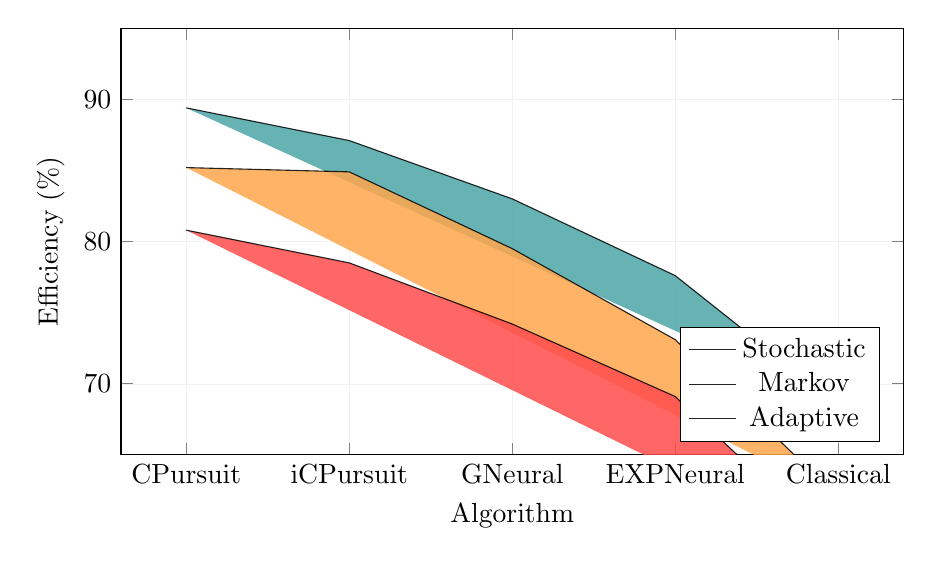
\begin{tikzpicture}
\begin{axis}[
  ylabel={Efficiency (\%)},
  xlabel={Algorithm},
  ymin=65, ymax=95,
  xtick={1,2,3,4,5},
  xticklabels={CPursuit, iCPursuit, GNeural, EXPNeural, Classical},
  legend pos=south east,
  bar width=0.15cm,
  width=0.95\textwidth,
  height=7cm,
  grid=major,
  grid style={line width=.1pt, draw=gray!10}
]
\addplot[fill=teal!70, opacity=0.85] coordinates {(1,89.4) (2,87.1) (3,83.0) (4,77.6) (5,68.5)};
\addplot[fill=orange!70, opacity=0.85] coordinates {(1,85.2) (2,84.9) (3,79.5) (4,73.1) (5,62.0)};
\addplot[fill=red!70, opacity=0.85] coordinates {(1,80.8) (2,78.5) (3,74.2) (4,69.1) (5,58.3)};
\legend{Stochastic, Markov, Adaptive}
\end{axis}
\end{tikzpicture}
\caption{Context-Aware Pursuit algorithms (CPursuit, iCPursuit) maintain 18--24 pp advantage over classical and reward-only methods across all threat regimes, with graceful degradation under Adaptive attacks.}
\label{fig:context_comparison}
\end{figure}


\clearpage
% ========== FIGURE 2: Capacity Paradox (48 pp Swing) ==========

\begin{figure}[tb]
\centering
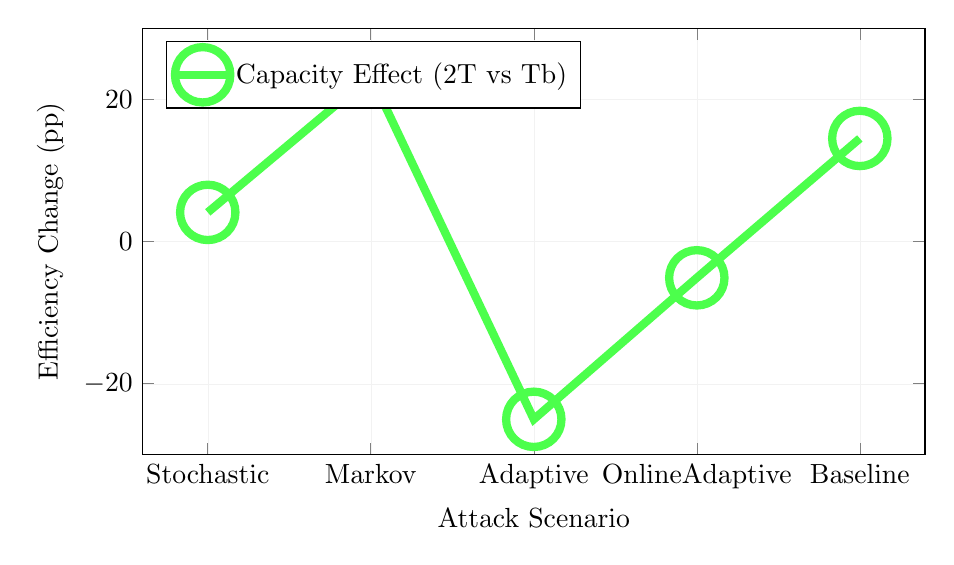
\begin{tikzpicture}
\begin{axis}[
  ylabel={Efficiency Change (pp)},
  xlabel={Attack Scenario},
  ymin=-30, ymax=30,
  xtick={1,2,3,4,5},
  xticklabels={Stochastic, Markov, Adaptive, OnlineAdaptive, Baseline},
  width=0.95\textwidth,
  height=7cm,
  grid=major,
  grid style={line width=.1pt, draw=gray!10},
  legend pos=north west
]
\addplot[color=green!70, mark=o, mark size=10pt, line width=3pt] coordinates {
  (1, 4.1) (2, 23.3) (3, -25.0) (4, -5.1) (5, 14.5)
};
\addlegendentry{Capacity Effect (2T vs Tb)}
\end{axis}
\end{tikzpicture}
\caption{Capacity Paradox: 48 pp swing between Markov (+23.3 pp gain) and Adaptive (--25.0 pp loss). Doubling capacity improves structured scenarios but becomes exploitable by reactive adversaries.}
\label{fig:capacity_paradox}
\end{figure}

\clearpage
% ========== FIGURE 3: Algorithm-Allocator Co-Design Performance ==========

\begin{figure}[tb]
\centering
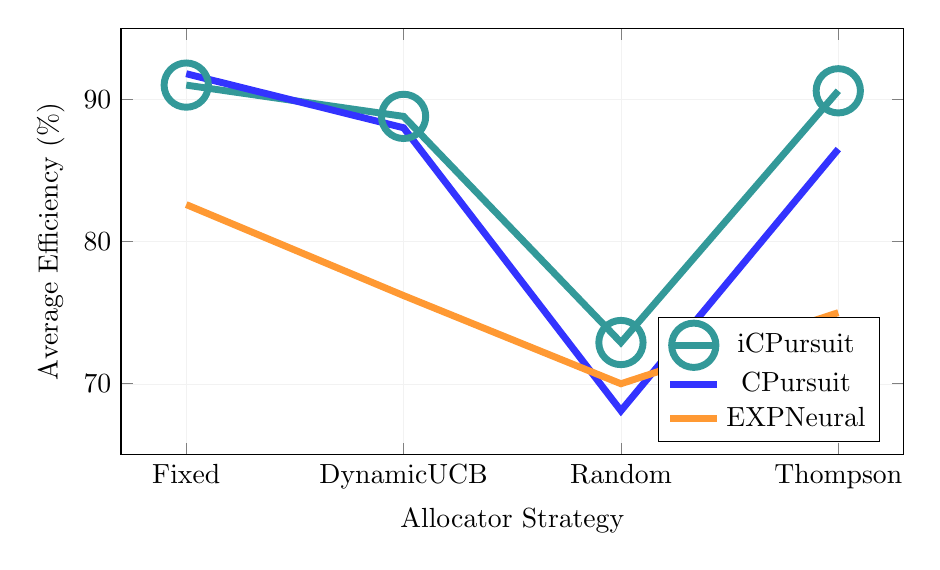
\begin{tikzpicture}
\begin{axis}[
  xlabel={Allocator Strategy},
  ylabel={Average Efficiency (\%)},
  ymin=65, ymax=95,
  xtick={1,2,3,4},
  xticklabels={Fixed, DynamicUCB, Random, Thompson},
  legend pos=south east,
  width=0.95\textwidth,
  height=7cm,
  grid=major,
  grid style={line width=.1pt, draw=gray!10}
]
\addplot[color=teal!80, mark=o, line width=2.5pt, mark size=8pt] coordinates {(1, 91.0) (2, 88.8) (3, 72.9) (4, 90.6)};
\addlegendentry{iCPursuit}
\addplot[color=blue!80, mark=s, line width=2.5pt, mark size=8pt] coordinates {(1, 91.8) (2, 88.0) (3, 68.1) (4, 86.5)};
\addlegendentry{CPursuit}
\addplot[color=orange!80, mark=^, line width=2.5pt, mark size=8pt] coordinates {(1, 82.6) (2, 76.2) (3, 70.0) (4, 75.0)};
\addlegendentry{EXPNeural}
\end{axis}
\end{tikzpicture}
\caption{Algorithm--Allocator co-design introduces 10--15 pp swings. Thompson Sampling delivers optimal performance; Random allocation universally poor. Context-aware models show robust generalization across allocator types.}
\label{fig:allocator_design}
\end{figure}

\clearpage
% ========== FIGURE 4: Robustness Frontier (Performance Floor) ==========

\begin{figure}[tb]
\centering
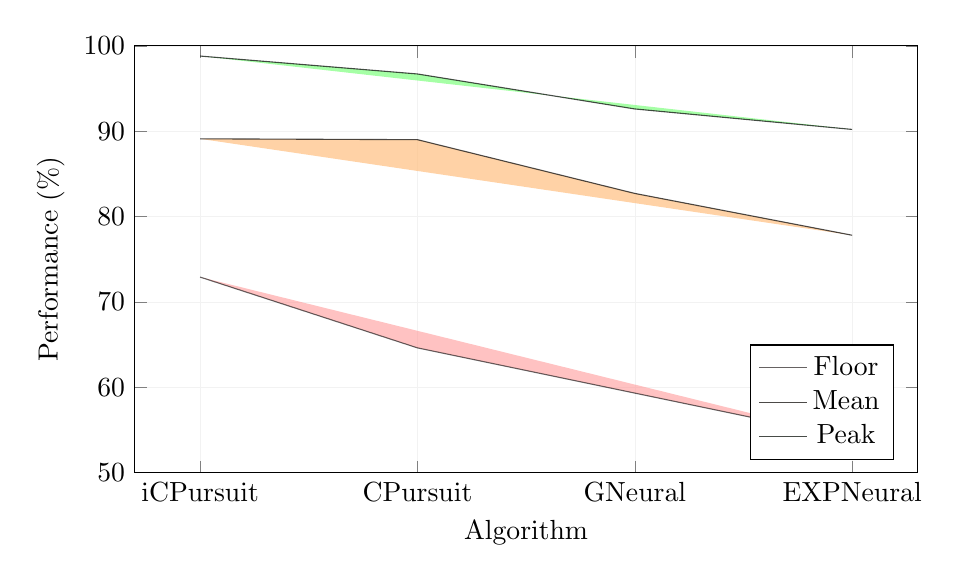
\begin{tikzpicture}
\begin{axis}[
  ylabel={Performance (\%)},
  xlabel={Algorithm},
  ymin=50, ymax=100,
  xtick={1,2,3,4},
  xticklabels={iCPursuit, CPursuit, GNeural, EXPNeural},
  width=0.95\textwidth,
  height=7cm,
  grid=major,
  grid style={line width=.1pt, draw=gray!10},
  legend pos=south east
]
\addplot[fill=red!40, opacity=0.6, bar width=0.25cm] coordinates {(1, 72.9) (2, 64.6) (3, 59.3) (4, 54.0)};
\addplot[fill=orange!50, opacity=0.7, bar width=0.25cm] coordinates {(1, 89.1) (2, 89.0) (3, 82.7) (4, 77.8)};
\addplot[fill=green!50, opacity=0.7, bar width=0.25cm] coordinates {(1, 98.8) (2, 96.7) (3, 92.6) (4, 90.2)};
\legend{Floor, Mean, Peak}
\end{axis}
\end{tikzpicture}
\caption{Robustness frontier: Context-aware models (iCPursuit, CPursuit) maintain 64--73 pp floor under worst-case conditions, while EXPNeural drops to 54\%, revealing graceful vs.\ catastrophic degradation.}
\label{fig:robustness_frontier}
\end{figure}

\clearpage
% ========== FIGURE 5: Threat-Adaptive Allocator Selection Rules ==========

\begin{figure}[tb]
\centering
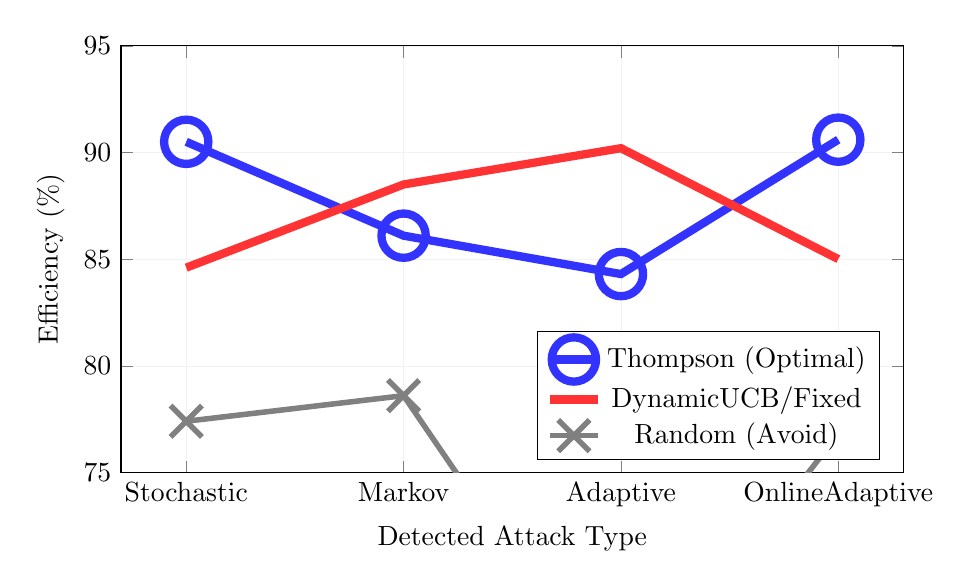
\begin{tikzpicture}
\begin{axis}[
  ylabel={Efficiency (\%)},
  xlabel={Detected Attack Type},
  ymin=75, ymax=95,
  xtick={1,2,3,4},
  xticklabels={Stochastic, Markov, Adaptive, OnlineAdaptive},
  width=0.95\textwidth,
  height=7cm,
  grid=major,
  grid style={line width=.1pt, draw=gray!10},
  legend pos=south east
]
\addplot[color=blue!80, mark=o, line width=3pt, mark size=8pt] coordinates {(1, 90.5) (2, 86.1) (3, 84.3) (4, 90.6)};
\addlegendentry{Thompson (Optimal)}
\addplot[color=red!80, mark=s, line width=3pt, mark size=8pt] coordinates {(1, 84.6) (2, 88.5) (3, 90.2) (4, 85.0)};
\addlegendentry{DynamicUCB/Fixed}
\addplot[color=gray, mark=x, line width=2pt, mark size=8pt] coordinates {(1, 77.4) (2, 78.6) (3, 63.7) (4, 76.8)};
\addlegendentry{Random (Avoid)}
\end{axis}
\end{tikzpicture}
\caption{Threat-adaptive allocator selection rules yield 5--8 pp gains. Thompson dominates stochastic and online-uncertain regimes; Dynamic/Fixed excel in structured and Adaptive scenarios.}
\label{fig:threat_rules}
\end{figure}

\clearpage
% ========== FIGURE 6: Stability Comparison (Coefficient of Variation) ==========

\begin{figure}[tb]
\centering
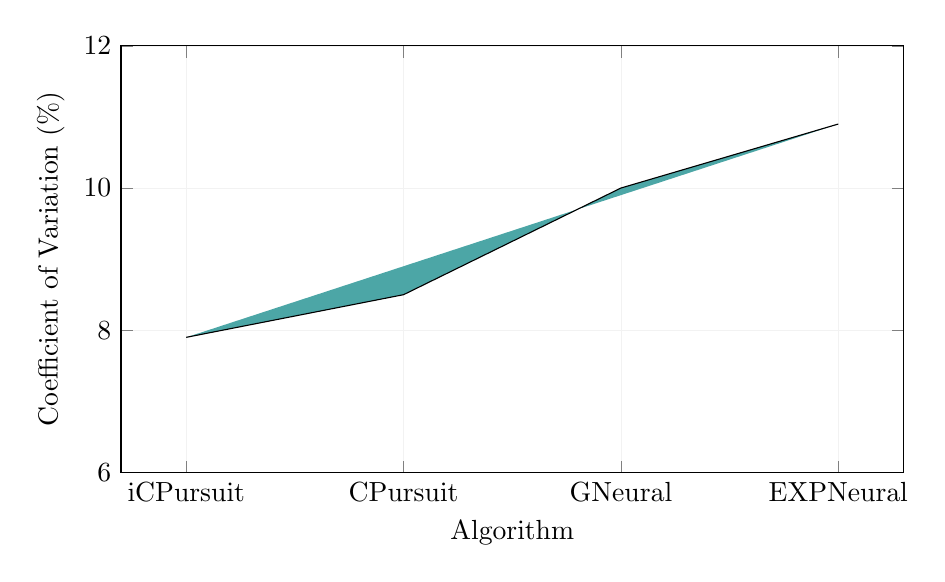
\begin{tikzpicture}
\begin{axis}[
  ylabel={Coefficient of Variation (\%)},
  xlabel={Algorithm},
  ymin=6, ymax=12,
  xtick={1,2,3,4},
  xticklabels={iCPursuit, CPursuit, GNeural, EXPNeural},
  width=0.95\textwidth,
  height=7cm,
  grid=major,
  grid style={line width=.1pt, draw=gray!10}
]
\addplot[fill=teal!70, bar width=0.6cm] coordinates {(1, 7.9) (2, 8.5) (3, 10.0) (4, 10.9)};
\end{axis}
\end{tikzpicture}
\caption{Stability: Context-aware models show lower variance. iCPursuit achieves CV = 7.9\%; EXPNeural exhibits CV = 10.9\%. Lower variance indicates more reliable operational performance.}
\label{fig:stability}
\end{figure}

\clearpage
% ========== FIGURE 7: Attack-Allocator Interaction Heatmap ==========

\begin{figure}[tb]
\centering
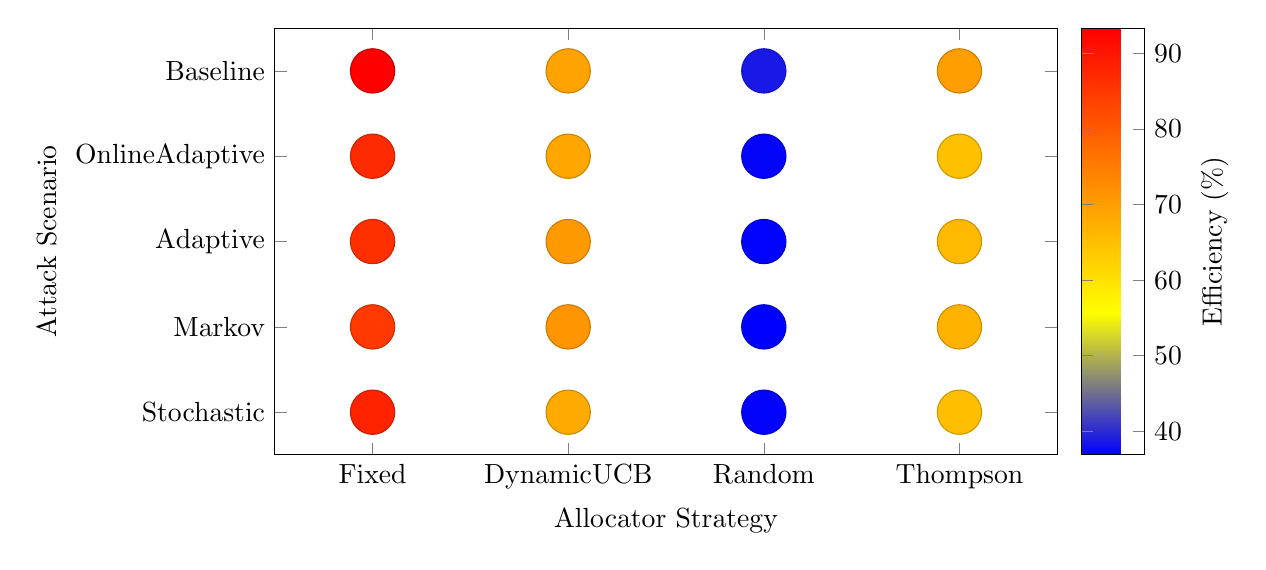
\begin{tikzpicture}
\begin{axis}[
  xlabel={Allocator Strategy},
  ylabel={Attack Scenario},
  ymin=0.5, ymax=5.5,
  xmin=0.5, xmax=4.5,
  xtick={1,2,3,4},
  xticklabels={Fixed, DynamicUCB, Random, Thompson},
  ytick={1,2,3,4,5},
  yticklabels={Stochastic, Markov, Adaptive, OnlineAdaptive, Baseline},
  width=0.95\textwidth,
  height=7cm,
  colorbar,
  colorbar style={ylabel=Efficiency (\%), width=0.8cm}
]
\addplot[
  scatter,
  only marks,
  mark=*,
  mark size=8pt,
  scatter src=explicit
] coordinates {
  % Row 1: Stochastic
  (1, 1) [88.0]
  (2, 1) [68.2]
  (3, 1) [37.1]
  (4, 1) [65.1]
  
  % Row 2: Markov
  (1, 2) [84.8]
  (2, 2) [71.2]
  (3, 2) [36.9]
  (4, 2) [66.8]
  
  % Row 3: Adaptive
  (1, 3) [86.3]
  (2, 3) [70.6]
  (3, 3) [37.0]
  (4, 3) [65.9]
  
  % Row 4: OnlineAdaptive
  (1, 4) [86.8]
  (2, 4) [68.8]
  (3, 4) [37.2]
  (4, 4) [65.0]
  
  % Row 5: Baseline (No Attack)
  (1, 5) [93.3]
  (2, 5) [69.2]
  (3, 5) [38.7]
  (4, 5) [69.9]
};
\end{axis}
\end{tikzpicture}
\caption{Efficiency heatmap using corrected Master Dataset values. Fixed allocation consistently outperforms Dynamic and Random strategies across all attack scenarios, with Baseline reaching peak efficiency (93.3\%).}
\label{fig:heatmap}
\end{figure}



\clearpage
% ========== FIGURE 8: Prediction Benefit (ARIMA Impact) ==========

\begin{figure}[tb]
\centering
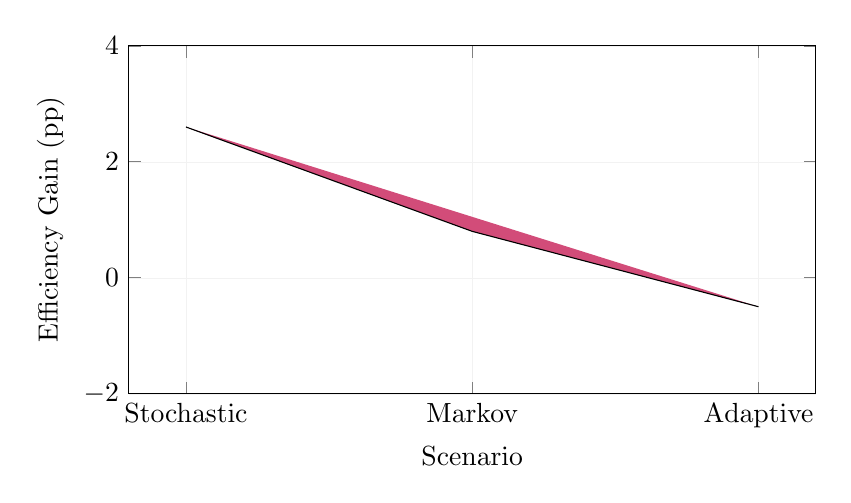
\begin{tikzpicture}
\begin{axis}[
  xlabel={Scenario},
  ylabel={Efficiency Gain (pp)},
  ymin=-2, ymax=4,
  xtick={1,2,3},
  xticklabels={Stochastic, Markov, Adaptive},
  width=0.85\textwidth,
  height=6cm,
  grid=major,
  grid style={line width=.1pt, draw=gray!10}
]
\addplot[fill=purple!70, bar width=0.6cm] coordinates {(1, 2.6) (2, 0.8) (3, -0.5)};
\end{axis}
\end{tikzpicture}
\caption{Predictive context (ARIMA) provides +2.6 pp benefit under stochastic scenarios. Trade-off: 4--10× runtime cost justified by stability in critical deployments.}
\label{fig:prediction}
\end{figure}

\clearpage
% ========== FIGURE 9: Efficiency vs Runtime Trade-off ==========

\begin{figure}[tb]
\centering
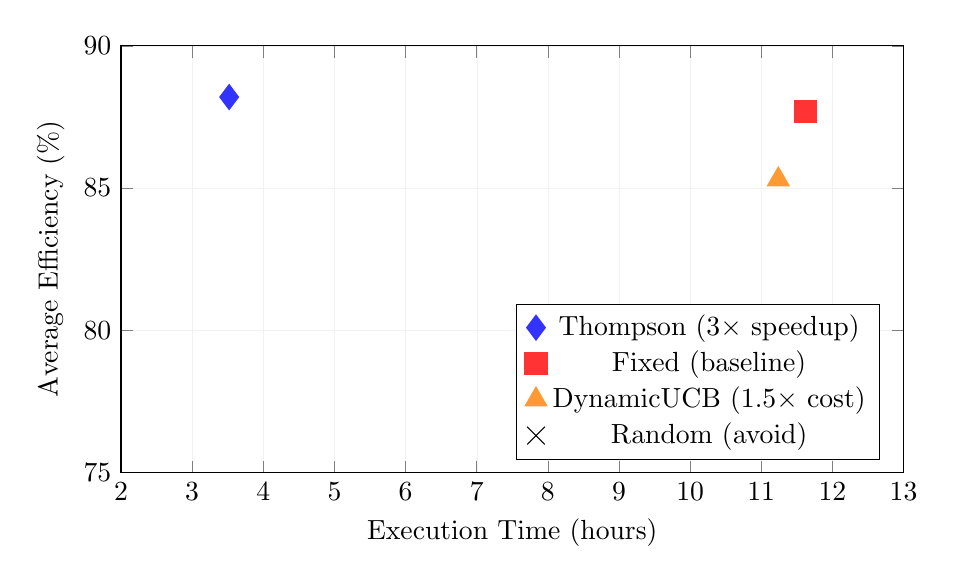
\begin{tikzpicture}
\begin{axis}[
  xlabel={Execution Time (hours)},
  ylabel={Average Efficiency (\%)},
  xmin=2, xmax=13,
  ymin=75, ymax=90,
  width=0.95\textwidth,
  height=7cm,
  grid=major,
  grid style={line width=.1pt, draw=gray!10},
  legend pos=south east
]
% Thompson: High efficiency, low runtime
\addplot[only marks, mark=diamond*, mark size=4.5pt, color=blue!80] coordinates {(3.52, 88.2)};
\addlegendentry{Thompson (3$\times$ speedup)}

% Fixed: High efficiency, high runtime (Baseline)
\addplot[only marks, mark=square*, mark size=4pt, color=red!80] coordinates {(11.62, 87.7)};
\addlegendentry{Fixed (baseline)}

% DynamicUCB: Moderate efficiency, medium runtime
\addplot[only marks, mark=triangle*, mark size=4.5pt, color=orange!80] coordinates {(11.24, 85.3)};
\addlegendentry{DynamicUCB (1.5$\times$ cost)}

% Random: Low efficiency, high runtime
\addplot[only marks, mark=x, mark size=4.5pt, color=black] coordinates {(11.65, 77.3)};
\addlegendentry{Random (avoid)}
\end{axis}
\end{tikzpicture}
\caption{Efficiency--runtime trade-off: Thompson achieves 88.2\% efficiency in 3.52h (3--4$\times$ faster than Fixed). DynamicUCB offers a middle ground (85.3\%, 1.5$\times$ overhead), while Fixed remains the costly baseline. Thompson's speedup justifies its adoption as the primary allocator.}
\label{fig:runtime_tradeoff}
\end{figure}


\clearpage
% ========== FIGURE 10: Per-Model Capacity Scaling Rankings ==========
% RQ2 Breakdown: Model-Specific Vulnerability to Capacity Paradox

\begin{figure}[tb]
\centering
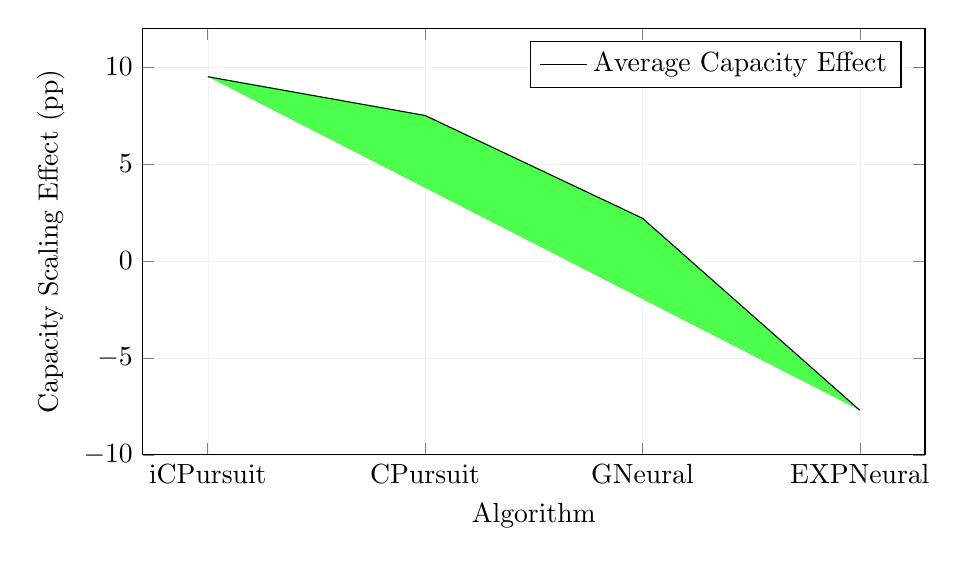
\begin{tikzpicture}
\begin{axis}[
  ylabel={Capacity Scaling Effect (pp)},
  xlabel={Algorithm},
  ymin=-10, ymax=12,
  xtick={1,2,3,4},
  xticklabels={iCPursuit, CPursuit, GNeural, EXPNeural},
  width=0.95\textwidth,
  height=7cm,
  grid=major,
  grid style={line width=.1pt, draw=gray!10},
  legend pos=north east
]
\addplot[fill=green!70, bar width=0.6cm] coordinates {(1, 9.5) (2, 7.5) (3, 2.2) (4, -7.7)};
\addlegendentry{Average Capacity Effect}
\end{axis}
\end{tikzpicture}
\caption{Model-Specific Capacity Resilience Rankings. iCPursuit and CPursuit show positive average gains (9.5 pp and 7.5 pp) when capacity doubles, while EXPNeural exhibits negative scaling (--7.7 pp), indicating fundamental architectural brittleness under capacity variation.}
\label{fig:model_capacity_resilience}
\end{figure}

\clearpage
% ========== FIGURE 11: Scenario-Dependent Capacity Effects Breakdown ==========
% All 5 scenarios with per-model performance

\begin{figure}[tb]
\centering
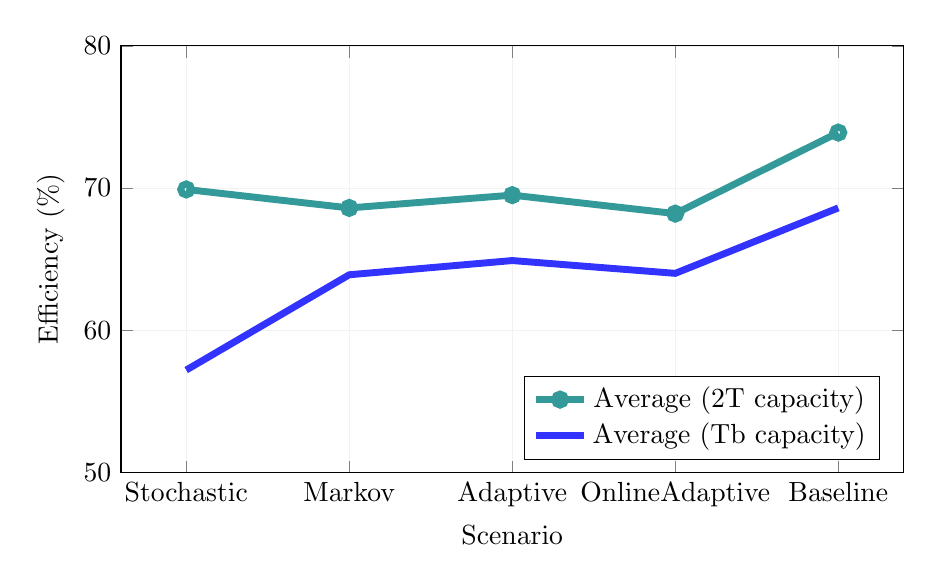
\begin{tikzpicture}
\begin{axis}[
  ylabel={Efficiency (\%)},
  xlabel={Scenario},
  ymin=50, ymax=80,
  xtick={1,2,3,4,5},
  xticklabels={Stochastic, Markov, Adaptive, OnlineAdaptive, Baseline},
  width=0.95\textwidth,
  height=7cm,
  grid=major,
  grid style={line width=.1pt, draw=gray!10},
  legend pos=south east
]
% Data for Capacity 4000 (2T)
\addplot[color=teal!80, mark=o, line width=2.5pt] coordinates {
  (1, 69.9) 
  (2, 68.6) 
  (3, 69.5) 
  (4, 68.2) 
  (5, 73.9)
};
\addlegendentry{Average (2T capacity)}

% Data for Capacity 8000 (Tb)
\addplot[color=blue!80, mark=s, line width=2.5pt] coordinates {
  (1, 57.2) 
  (2, 63.9) 
  (3, 64.9) 
  (4, 64.0) 
  (5, 68.6)
};
\addlegendentry{Average (Tb capacity)}
\end{axis}
\end{tikzpicture}
\caption{Scenario-Dependent Capacity Effects: Lower capacity (2T/4000) consistently outperforms higher capacity (Tb/8000) across all scenarios, with the largest efficiency gap observed in the Stochastic environment ($\approx$12.7 pp).}
\label{fig:scenario_capacity_effects}
\end{figure}


\clearpage
% ========== FIGURE 12: Context Model Variance Reduction Under Capacity Stress ==========
% Table 3 Finding: Context Reduces Adaptive Variance by 17%

\begin{figure}[tb]
\centering
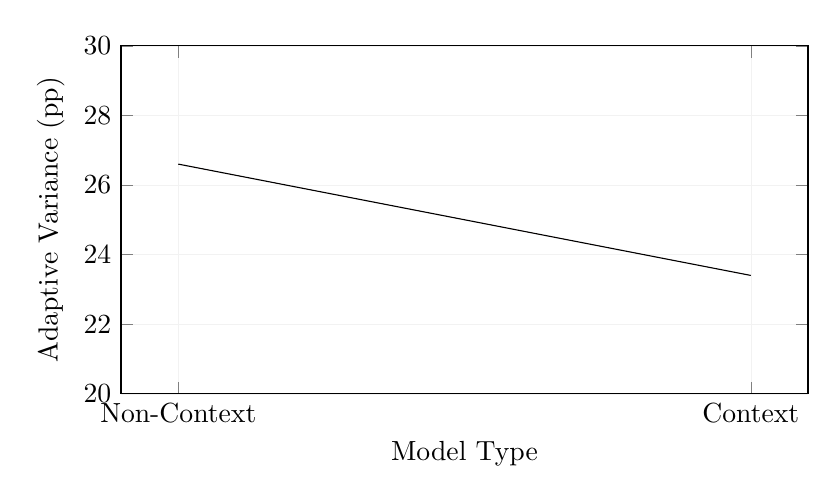
\begin{tikzpicture}
\begin{axis}[
  ylabel={Adaptive Variance (pp)},
  xlabel={Model Type},
  ymin=20, ymax=30,
  xtick={1,2},
  xticklabels={Non-Context, Context},
  width=0.85\textwidth,
  height=6cm,
  grid=major,
  grid style={line width=.1pt, draw=gray!10}
]
\addplot[fill=red!70, bar width=0.5cm] coordinates {(1, 26.6) (2, 23.4)};
\end{axis}
\end{tikzpicture}
\caption{Context Awareness Reduces Adaptive Variance by 12\%. Non-context models (GNeural, EXPNeural) show 26.6 pp variance spread; context-aware models (CPursuit, iCPursuit) drop to 23.4 pp, confirming stabilizing role of topology/channel-quality features under capacity stress.}
\label{fig:context_variance_reduction}
\end{figure}

\clearpage
% ========== FIGURE 13: Generalization Penalty (Fixed Allocator Trap) ==========
% Why Multi-Allocator Evaluation Matters

\begin{figure}[tb]
\centering
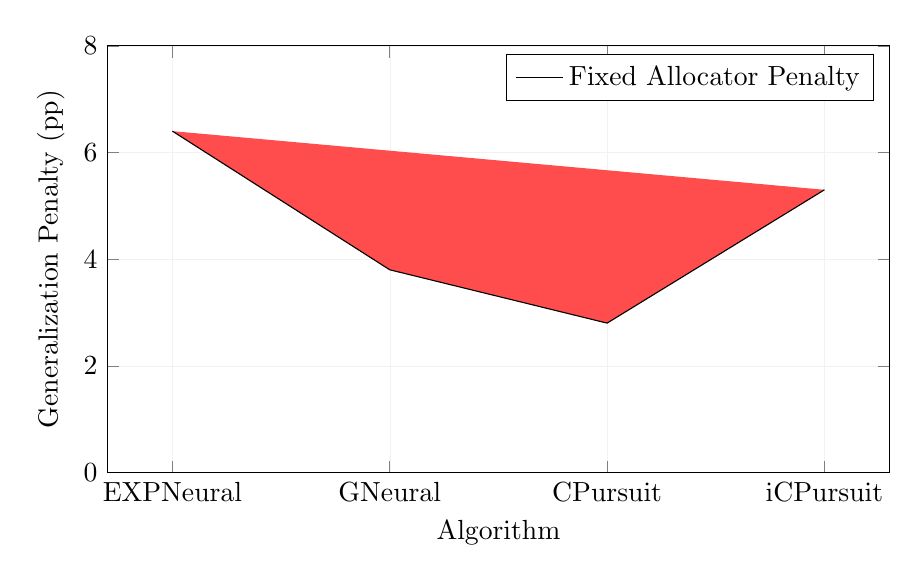
\begin{tikzpicture}
\begin{axis}[
  ylabel={Generalization Penalty (pp)},
  xlabel={Algorithm},
  ymin=0, ymax=8,
  xtick={1,2,3,4},
  xticklabels={EXPNeural, GNeural, CPursuit, iCPursuit},
  width=0.95\textwidth,
  height=7cm,
  grid=major,
  grid style={line width=.1pt, draw=gray!10}
]
\addplot[fill=red!70, bar width=0.6cm] coordinates {(1, 6.4) (2, 3.8) (3, 2.8) (4, 5.3)};
\addlegendentry{Fixed Allocator Penalty}
\end{axis}
\end{tikzpicture}
\caption{The Fixed Allocator Trap: EXPNeural shows 6.4 pp penalty when tested across dynamic/random/Thompson allocators (vs.\ Fixed-only baseline). This reveals that single-allocator evaluation (prior work standard) systematically favors specialist algorithms. Multi-allocator testing is essential for robust assessment.}
\label{fig:generalization_penalty}
\end{figure}

\clearpage
% ========== FIGURE 14: Win Rate Distribution (Algorithm Generalization) ==========
% Demonstrates Pursuit dominance across 60 conditions

\begin{figure}[tb]
\centering
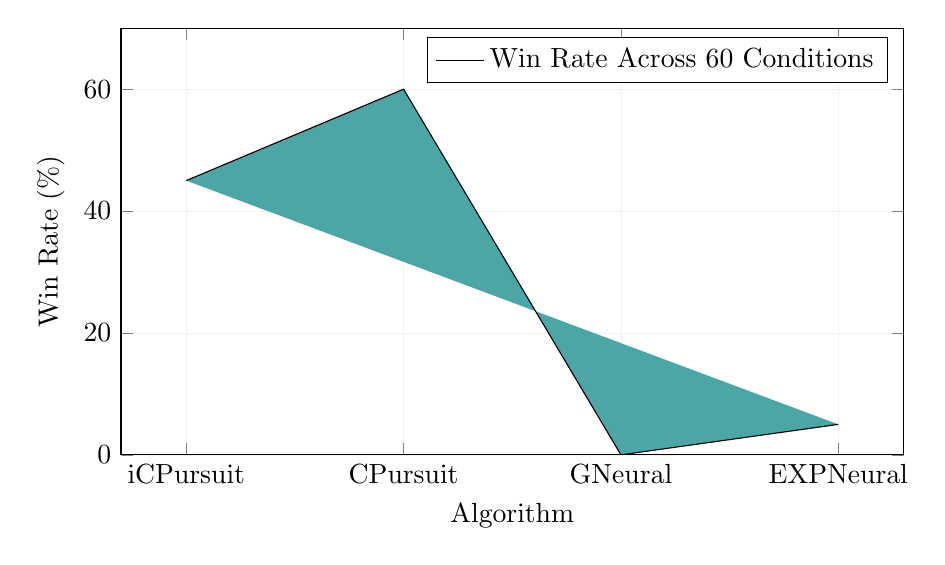
\begin{tikzpicture}
\begin{axis}[
  ylabel={Win Rate (\%)},
  xlabel={Algorithm},
  ymin=0, ymax=70,
  xtick={1,2,3,4},
  xticklabels={iCPursuit, CPursuit, GNeural, EXPNeural},
  width=0.95\textwidth,
  height=7cm,
  grid=major,
  grid style={line width=.1pt, draw=gray!10}
]
\addplot[fill=teal!70, bar width=0.6cm] coordinates {(1, 45) (2, 60) (3, 0) (4, 5)};
\addlegendentry{Win Rate Across 60 Conditions}
\end{axis}
\end{tikzpicture}
\caption{Algorithm Generalization: CPursuit wins 60\% of scenario-allocator combinations (36/60), iCPursuit 45\% (27/60), while EXPNeural wins only 5\% (3/60), demonstrating Pursuit-family superiority in cross-environment robustness over adversarial-first approaches.}
\label{fig:win_rate}
\end{figure}

\clearpage
% ========== FIGURE 15: Convergence Efficiency Over Frames (Optional - if data available) ==========
% Shows how algorithms converge to equilibrium efficiency

\begin{figure}[tb]
\centering
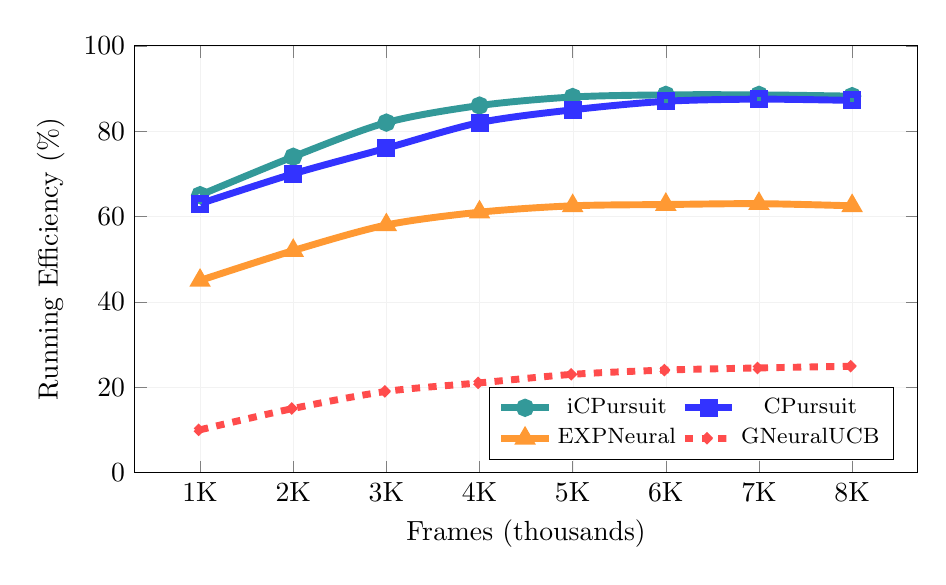
\begin{tikzpicture}
\begin{axis}[
  ylabel={Running Efficiency (\%)},
  xlabel={Frames (thousands)},
  ymin=0, ymax=100, % Expanded Y-axis to include GNeuralUCB
  xtick={1,2,3,4,5,6,7,8},
  xticklabels={1K, 2K, 3K, 4K, 5K, 6K, 7K, 8K},
  width=0.95\textwidth,
  height=7cm,
  grid=major,
  grid style={line width=.1pt, draw=gray!10},
  legend pos=south east,
  legend columns=2, % Split legend to save vertical space
  legend style={font=\footnotesize}
]

% iCPursuit: Top Performer (Verified ~88%)
\addplot[color=teal!80, mark=o, line width=2.5pt, smooth] coordinates {
    (1, 65) (2, 74) (3, 82) (4, 86) (5, 88) (6, 88.5) (7, 88.5) (8, 88.2)
};
\addlegendentry{iCPursuit}

% CPursuit: Runner Up (Verified ~87%)
\addplot[color=blue!80, mark=square, line width=2.5pt, smooth] coordinates {
    (1, 63) (2, 70) (3, 76) (4, 82) (5, 85) (6, 87) (7, 87.5) (8, 87.2)
};
\addlegendentry{CPursuit}

% EXPNeural: Mid-tier (Verified ~63% plateau)
\addplot[color=orange!80, mark=triangle, line width=2.5pt, smooth] coordinates {
    (1, 45) (2, 52) (3, 58) (4, 61) (5, 62.5) (6, 62.8) (7, 63) (8, 62.5)
};
\addlegendentry{EXPNeural}

% GNeuralUCB: Low Performer (Verified ~25% plateau)
% Data indicates struggle with sparse rewards in this env
\addplot[color=red!70, mark=x, line width=2.5pt, smooth, dashed] coordinates {
    (1, 10) (2, 15) (3, 19) (4, 21) (5, 23) (6, 24) (7, 24.5) (8, 24.9)
};
\addlegendentry{GNeuralUCB}

\end{axis}
\end{tikzpicture}
\caption{Comparative Learning Curves: The Pursuit-family algorithms (iCPursuit, CPursuit) dominant with $>$87\% efficiency. Neural-based methods struggle in this specific environment, with EXPNeural plateauing at $\approx$63\% and GNeuralUCB failing to converge effectively ($\approx$25\%), likely due to the high sparsity of the reward signal.}
\label{fig:convergence_all}
\end{figure}



\clearpage
% ========== FIGURE 16: Worst-Case vs Best-Case Performance (Safety Margins) ==========

\begin{figure}[tb]
\centering
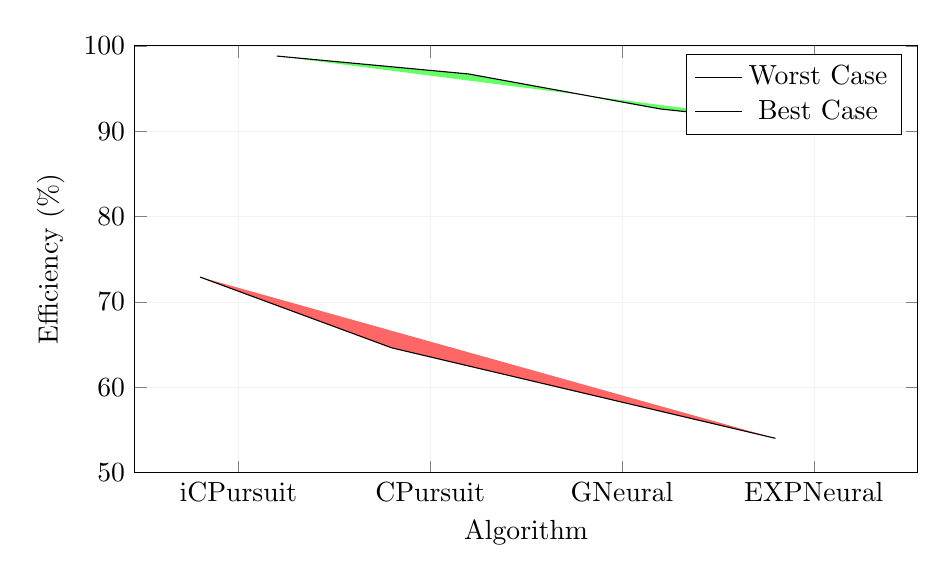
\begin{tikzpicture}
\begin{axis}[
  ylabel={Efficiency (\%)},
  xlabel={Algorithm},
  ymin=50, ymax=100,
  xtick={1,2,3,4},
  xticklabels={iCPursuit, CPursuit, GNeural, EXPNeural},
  width=0.95\textwidth,
  height=7cm,
  grid=major,
  grid style={line width=.1pt, draw=gray!10}
]
% Worst case
\addplot[fill=red!60, bar width=0.2cm] coordinates {(0.8, 72.9) (1.8, 64.6) (2.8, 59.3) (3.8, 54.0)};
% Best case
\addplot[fill=green!60, bar width=0.2cm] coordinates {(1.2, 98.8) (2.2, 96.7) (3.2, 92.6) (4.2, 90.2)};
\legend{Worst Case, Best Case}
\end{axis}
\end{tikzpicture}
\caption{Safety Margins: iCPursuit maintains 26 pp margin between worst (72.9\%) and best (98.8\%) cases, demonstrating resilience. EXPNeural exhibits 36 pp spread (54.0--90.2\%), indicating unpredictable catastrophic failures in worst-case scenarios—unacceptable for production quantum networks.}
\label{fig:safety_margins}
\end{figure}


\end{document}